\documentclass[10pt]{beamer}

%%%
% PREAMBLE FOR THIS DOC 
%%%
%https://tex.stackexchange.com/questions/68821/is-it-possible-to-create-a-latex-preamble-header
\usepackage{/Users/miw267/Repos/csci246_spring2025/slides/preambles/beamer_preamble_for_CSCI246}

\usetikzlibrary{matrix}

\usetikzlibrary{shapes.geometric}

\usepackage{pgfplots} % For drawing histograms
\usetikzlibrary{pgfplots.groupplots} % For grouping multiple plots


%%% TRY TO RESHOW TOC AT EACH SECTION START (with current section highlighted)
% Reference: https://tex.stackexchange.com/questions/280436/how-to-highlight-a-specific-section-in-beamer-toc
\newcommand\tocforsect[2]{%
  \begingroup
  \edef\safesection{\thesection}
  \setcounter{section}{#1}
  \tableofcontents[#2,currentsection]
  \setcounter{section}{\safesection}
  \endgroup
}


%%%% HERES HOW TO DO IT CORRECTLY
% FIRST IN .STY FILE, DO
%\usetheme[sectionpage=none]{metropolis}
% THEN AT EACH SECTION DO
%\begin{frame}{Outline}
%  \tableofcontents[currentsection]	
%\end{frame}



%\setbeamertemplate{navigation symbols}{}
%\setbeamertemplate{footline}[frame number]{}


%%%
% DOCUMENT
%%%

\begin{document}

%\maketitle

%% Title page frame
%\begin{frame}
%    \titlepage 
%\end{frame}



\title{03/31/2025: Expectation}
\author{CSCI 246: Discrete Structures}
\date{Textbook reference: Sec 34, Scheinerman}

\begin{frame}
    \titlepage 
\end{frame}


\begin{frame}
\small
\begin{mygreenbox}[title=Graded Quiz Pickup]
Quizzes are in the front of the room, grouped into four bins (A-G, H-L, M-R, S-Z) by last name. The quizzes are upside down with your last name on the back. Come find yours before, during, or after class. Only turn the quiz over if it's yours. \\ 

%\textbf{Alert.} Some of you weren't here the Friday before spring break. These stacks also include uncollected reading quizzes from Wed. Mar 12 -- Intro to Probability (Part 1). 
\end{mygreenbox} 
\vfill 

\begin{myredbox}[title=Today's Agenda]
\begin{itemize}
	\item Reading quiz (5 mins)
	\item Mini-lecture ($\approx$ 20 mins)
	\item Group exercises ($\approx$ 20 mins)
\end{itemize}


\end{myredbox}
\vfill 

\end{frame}






\begin{frame}[standout]
Feedback on Friday's Quizzes
\end{frame}

\begin{frame}{Reading Quiz Scores}
\footnotesize 
\begin{figure}[ht]
        \centering
        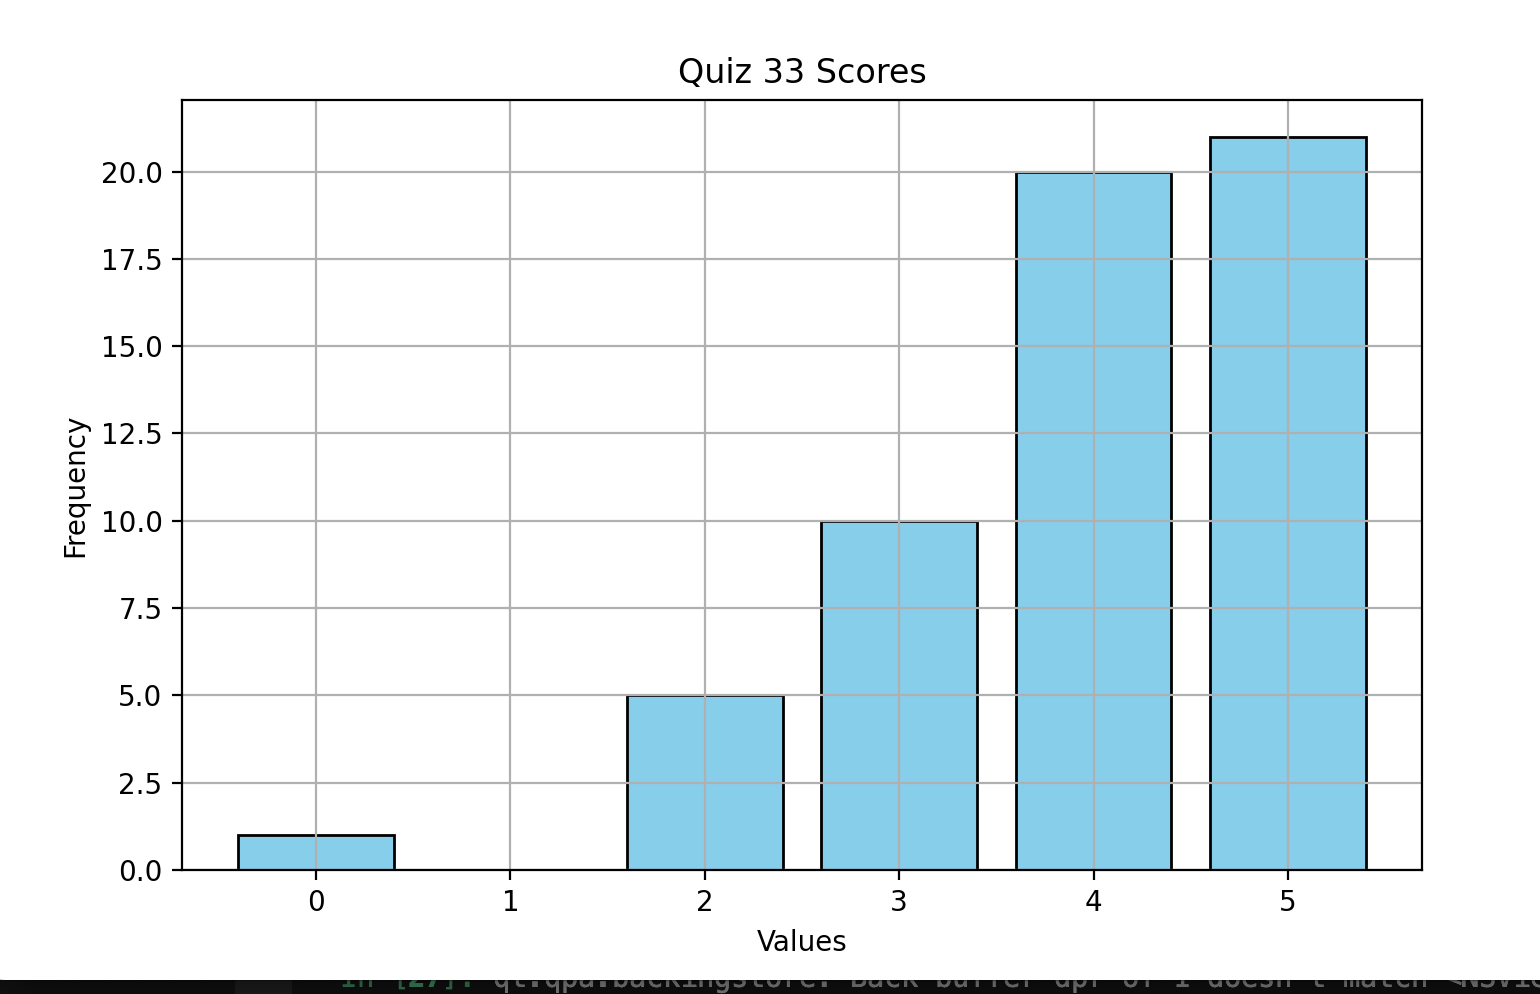
\includegraphics[width=.8\textwidth]{images/reading_quiz_scores}
   		 \caption{Median Score = 4/5 (80\%)}
\end{figure}
\vfill 
\textbf{Grading Rubric.}  	
\begin{enumerate}
\item 1 point for stating that a \textit{random variable} is a function on the sample space $S$. 
\item 4 points (1 per subpart). Correct answers: True, True, True, True.
\end{enumerate}

\end{frame}	

\begin{frame}{Problem Quiz Scores}
\footnotesize 
\begin{figure}[ht]
        \centering
        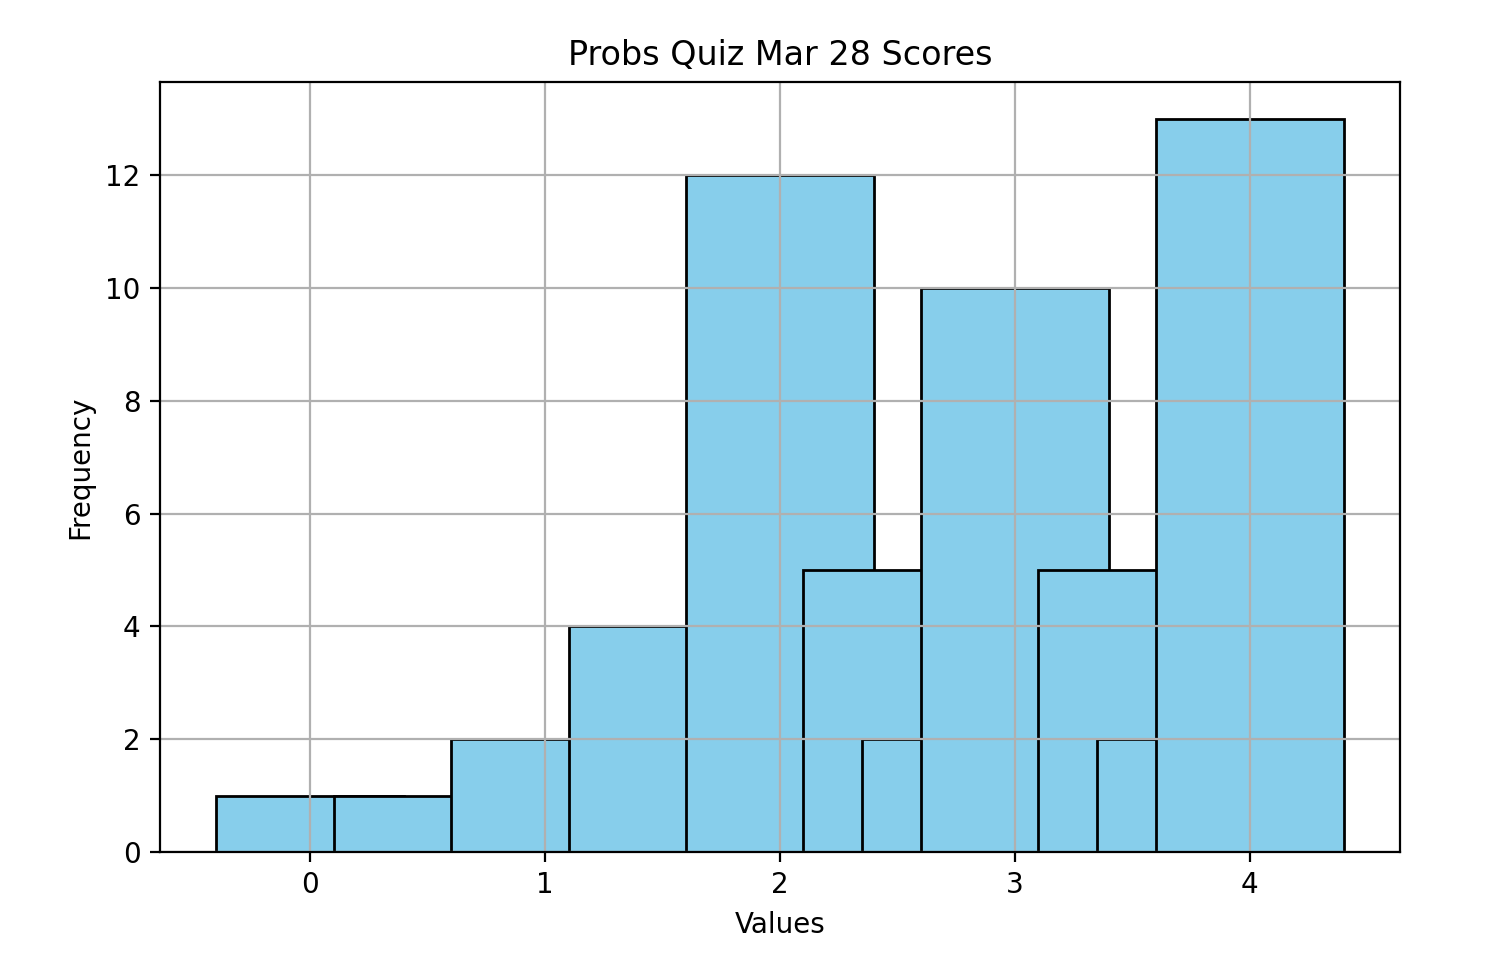
\includegraphics[width=.8\textwidth]{images/problems_quiz_scores}
   		 \caption{Median Score = 3/4 (75\%)}
\end{figure}
\vfill 
\textbf{Grading Rubric.}  
\begin{enumerate}
\item 2 points for correctly providing the \# of subsets in 2 different ways.
\item 2 points for correctly providing the probability of a full house. (\alert{Let's review this.}) 
\end{enumerate} 
\end{frame}	




\begin{frame}[standout]
Today's quiz
\end{frame}

\begin{frame}
\small 

\begin{myredbox}[title=\text{Reading Quiz (Expectation)}]

Answer the questions below.  You do \textbf{not} need to simplify your answers! \\

\begin{minipage}{.7\textwidth}
\begin{enumerate}
	\item Consider the spinner shown in the figure. Suppose that the likelihood of landing in each region is proportional to the area of the region.  Let $X$ be the number that appears on the spinner. Compute the expected value of $X$.
	\item (Extra credit.) Let $X$ be the number that appears on a random toss of a die.  Compute the variance of $X$.
\end{enumerate}
\end{minipage} %
\hfill 
\begin{minipage}{.28\textwidth}
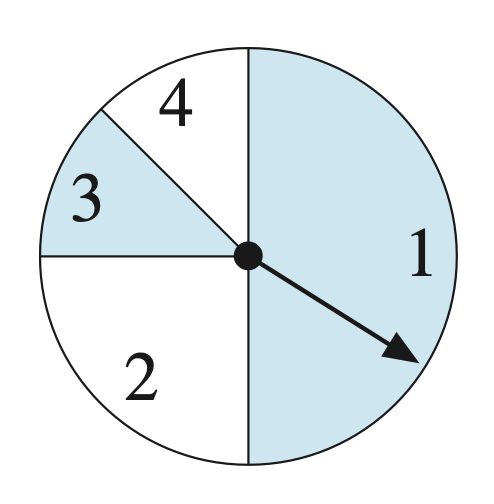
\includegraphics[width=\textwidth]{images/spinner.png}
\end{minipage}

\end{myredbox}
	
\end{frame}



\begin{frame}[standout]
Thoughts on Expectation
\end{frame}





\begin{frame}

Suppose we roll a pair of dice.  What is the \textit{expected value} of the sum?
\vfill 
\begin{figure}

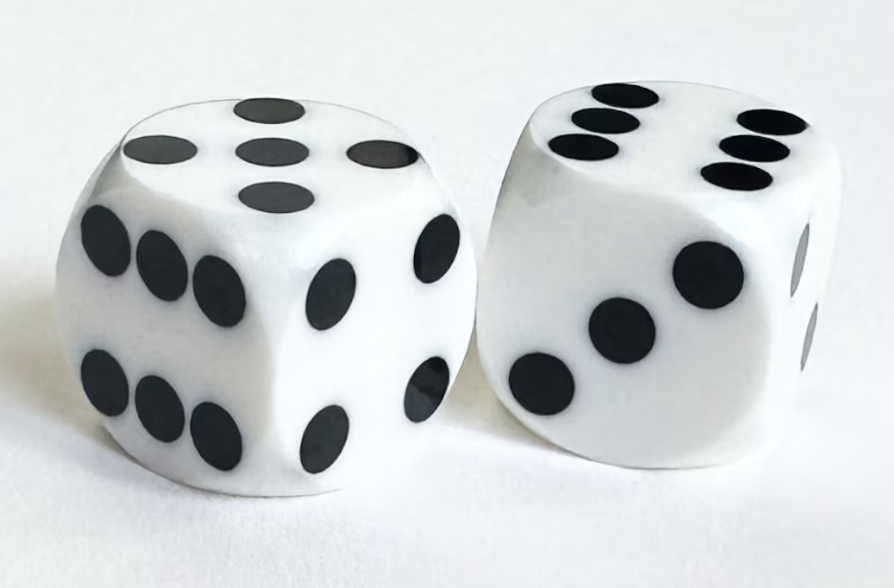
\includegraphics[width=.8\textwidth]{images/pair_of_dice.png}
\end{figure}
\vfill 
Formally, let $X$ be the sum of the number on the two dice.  We must compute $E[X]$.
	
\end{frame}

\begin{frame}{Computing An Expectation}
\footnotesize 
\begin{table}
\caption{\textit{Possible outcomes when rolling a pair of dice.} Each table entry gives the sum of the values on the two dice.}	
\pause 
\resizebox{0.6\textwidth}{!}{%
\begin{tabular}{|c|c|c|c|c|c|c|c|}
\hline
\textbf{Dice Values} & \textbf{1} & \textbf{2} & \textbf{3} & \textbf{4} & \textbf{5} & \textbf{6} \\
\hline
\textbf{1} & \cellcolor{red!20} 2  & \cellcolor{red!40} 3  & \cellcolor{red!60} 4  & \cellcolor{red!80} 5  & \cellcolor{red!90} 6  & \cellcolor{red!100} 7 \\
\hline
\textbf{2} & \cellcolor{red!40} 3  & \cellcolor{red!60} 4  & \cellcolor{red!80} 5  & \cellcolor{red!90} 6  & \cellcolor{red!100} 7  & \cellcolor{orange!80} 8 \\
\hline
\textbf{3} & \cellcolor{red!60} 4  & \cellcolor{red!80} 5  & \cellcolor{red!90} 6  & \cellcolor{red!100} 7  & \cellcolor{orange!80} 8  & \cellcolor{orange!60} 9 \\
\hline
\textbf{4} & \cellcolor{red!80} 5  & \cellcolor{red!90} 6  & \cellcolor{red!100} 7  & \cellcolor{orange!80} 8  & \cellcolor{orange!60} 9  & \cellcolor{orange!40} 10 \\
\hline
\textbf{5} & \cellcolor{red!90} 6  & \cellcolor{red!100} 7  & \cellcolor{orange!80} 8  & \cellcolor{orange!60} 9  & \cellcolor{orange!40} 10 & \cellcolor{orange!20} 11 \\
\hline
\textbf{6} & \cellcolor{red!100} 7 & \cellcolor{orange!80} 8 & \cellcolor{orange!60} 9 & \cellcolor{orange!40} 10 & \cellcolor{orange!20} 11 & \cellcolor{yellow!20} 12 \\
\hline
\end{tabular}
}
\end{table}

\vfill 
\colorbox{blue!30}{\textbf{Method 1.}} \pause \; Sum over outcomes in the sample space.
\[ E[X] = \sum_{s \in S} X(s) P(s) \]
\vfill 
\pause 
\colorbox{blue!30}{\textbf{Application.}}
\scriptsize 
\begin{align*}
 E[X] 
&=\colorbox{red!20}{1+1} \!\cdot\! \frac{1}{36} + \colorbox{red!40}{1+2}\!\cdot\!\frac{1}{36}  + \colorbox{red!40}{2+1} \!\cdot\! \frac{1}{36} +\colorbox{red!60}{3+1} \!\cdot\! \frac{1}{36}  + \colorbox{red!60}{2+2} \!\cdot\!\frac{1}{36}  + 
 \colorbox{red!60}{1+3} \!\cdot\!\frac{1}{36} + \hdots + 
  \colorbox{yellow!20}{6+6} \!\cdot\! \frac{1}{36}  \\
 &= \colorbox{red!20}{2} \cdot \frac{1}{36} + \colorbox{red!40}{3} \cdot \frac{1}{36}  + \colorbox{red!40}{3} \cdot \frac{1}{36} +\colorbox{red!60}{4} \cdot \frac{1}{36}  + \colorbox{red!60}{4} \cdot \frac{1}{36}  + 
 \colorbox{red!60}{4} \cdot \frac{1}{36} + \hdots + 
  \colorbox{yellow!20}{12} \cdot \frac{1}{36} 
\end{align*}
\footnotesize 
\vfill 
\pause 
\colorbox{blue!30}{\textbf{Remark.}} \; We must sum over \textbf{many} (36) terms.
\end{frame}


\begin{frame}{Computing An Expectation}
\footnotesize  
\begin{table}
\caption{\textit{Possible outcomes when rolling a pair of dice.} Each table entry gives the sum of the values on the two dice.}	
\begin{tabular}{|c|c|c|c|c|c|c|c|}
\hline
\textbf{Dice Values} & \textbf{1} & \textbf{2} & \textbf{3} & \textbf{4} & \textbf{5} & \textbf{6} \\
\hline
\textbf{1} & \cellcolor{red!20} 2  & \cellcolor{red!40} 3  & \cellcolor{red!60} 4  & \cellcolor{red!80} 5  & \cellcolor{red!90} 6  & \cellcolor{red!100} 7 \\
\hline
\textbf{2} & \cellcolor{red!40} 3  & \cellcolor{red!60} 4  & \cellcolor{red!80} 5  & \cellcolor{red!90} 6  & \cellcolor{red!100} 7  & \cellcolor{orange!80} 8 \\
\hline
\textbf{3} & \cellcolor{red!60} 4  & \cellcolor{red!80} 5  & \cellcolor{red!90} 6  & \cellcolor{red!100} 7  & \cellcolor{orange!80} 8  & \cellcolor{orange!60} 9 \\
\hline
\textbf{4} & \cellcolor{red!80} 5  & \cellcolor{red!90} 6  & \cellcolor{red!100} 7  & \cellcolor{orange!80} 8  & \cellcolor{orange!60} 9  & \cellcolor{orange!40} 10 \\
\hline
\textbf{5} & \cellcolor{red!90} 6  & \cellcolor{red!100} 7  & \cellcolor{orange!80} 8  & \cellcolor{orange!60} 9  & \cellcolor{orange!40} 10 & \cellcolor{orange!20} 11 \\
\hline
\textbf{6} & \cellcolor{red!100} 7 & \cellcolor{orange!80} 8 & \cellcolor{orange!60} 9 & \cellcolor{orange!40} 10 & \cellcolor{orange!20} 11 & \cellcolor{yellow!20} 12 \\
\hline
\end{tabular}
\end{table}

\vfill 

\colorbox{blue!30}{\textbf{Method 2.}} \pause  Sum over possible values of the random variable.
\[ E[X] = \sum_{a \in \R} a \; P(X=a) \]
\vfill 
\pause 
\colorbox{blue!30}{\textbf{Application.}}
\begin{align*}
 E[X] &= \colorbox{red!20}{2} \cdot \frac{1}{36} + \colorbox{red!40}{3} \cdot \frac{2}{36}  +\colorbox{red!60}{4} \cdot \frac{3}{36}  +\hdots + 
  \colorbox{yellow!20}{12} \cdot \frac{1}{36} 
\end{align*}
\vfill 
\pause 
\colorbox{blue!30}{\textbf{Remark.}} \; We must sum over \textbf{fewer} (12) terms.
\end{frame}


\begin{frame}{Computing An Expectation}
\footnotesize  
\begin{table}
\caption{\textit{Possible outcomes when rolling a pair of dice.} Each table entry gives the sum of the values on the two dice.}	
\begin{tabular}{|c|c|c|c|c|c|c|c|}
\hline
\textbf{Dice Values} & \textbf{1} & \textbf{2} & \textbf{3} & \textbf{4} & \textbf{5} & \textbf{6} \\
\hline
\textbf{1} & \cellcolor{red!20} 2  & \cellcolor{red!40} 3  & \cellcolor{red!60} 4  & \cellcolor{red!80} 5  & \cellcolor{red!90} 6  & \cellcolor{red!100} 7 \\
\hline
\textbf{2} & \cellcolor{red!40} 3  & \cellcolor{red!60} 4  & \cellcolor{red!80} 5  & \cellcolor{red!90} 6  & \cellcolor{red!100} 7  & \cellcolor{orange!80} 8 \\
\hline
\textbf{3} & \cellcolor{red!60} 4  & \cellcolor{red!80} 5  & \cellcolor{red!90} 6  & \cellcolor{red!100} 7  & \cellcolor{orange!80} 8  & \cellcolor{orange!60} 9 \\
\hline
\textbf{4} & \cellcolor{red!80} 5  & \cellcolor{red!90} 6  & \cellcolor{red!100} 7  & \cellcolor{orange!80} 8  & \cellcolor{orange!60} 9  & \cellcolor{orange!40} 10 \\
\hline
\textbf{5} & \cellcolor{red!90} 6  & \cellcolor{red!100} 7  & \cellcolor{orange!80} 8  & \cellcolor{orange!60} 9  & \cellcolor{orange!40} 10 & \cellcolor{orange!20} 11 \\
\hline
\textbf{6} & \cellcolor{red!100} 7 & \cellcolor{orange!80} 8 & \cellcolor{orange!60} 9 & \cellcolor{orange!40} 10 & \cellcolor{orange!20} 11 & \cellcolor{yellow!20} 12 \\
\hline
\end{tabular}
\end{table}

\vfill 
\colorbox{blue!30}{\textbf{Method 3.}}\pause  Use linearity of expectation.
\[ E[X] = E[D_1] + E[D_2] \]
where $D_n$ is the value on the $n$-th die.
\vfill 
\pause 
\colorbox{blue!30}{\textbf{Application.}} We have 
\begin{align*}
 E[X] &= E[D_1] + E[D_2] = 3.5 + 3.5 = 7.
\end{align*}
%
since, by the previous methods, each $E[D_n] = \frac{1}{6} \cdot  (1+2+3+4+5+6) = 3.5$.

\vfill 
\pause 
\colorbox{blue!30}{\textbf{Remark.}} \; Here we can sum over \textbf{even fewer} (7) terms.   (Note: we can only use Method 3 in cases where we can express $X$ as a sum of other RVs).
\end{frame}


\begin{frame}{Summary on computing an expectation}
Some ways of computing the expectation are more efficient than others.
\vfill 
Foreshadowing our upcoming section on computational complexity, we can make a more general statement: 
\vfill 

\begin{myredbox}[title=\text{Remark: Scalability of different methods for computing an expectation}]
Let $X$ be the sum of $n$ random variables each from the same sample space $S$.  Then the number of operations needed to compute $E[X]$ is
\vfill 
\begin{itemize}
\item Method 1: $\mathcal{O}(|S|^n)$	, i.e. \textbf{exponential} in $n$.
\item Method 2: $\mathcal{O}(n \, |S|)$, i.e. \textbf{linear} in $n$.
\item Method 3: $\mathcal{O}(|S|)$,  i.e. \textbf{independent} of $n$.
\end{itemize}
\end{myredbox}

We will investigate computational complexity (and define $\mathcal{O}$) in a couple of class meetings.

\end{frame}


\begin{frame}{Expectation as center of probability mass}
\footnotesize 
Consider a probability space $(S,P)$ where $S=\set{1,2,\hdots,10}$ and $P(s) =\frac{1}{10}$ for all outcomes $s \in S$.  Define a random variable $X$ as below:
\vfill 
\begin{figure}
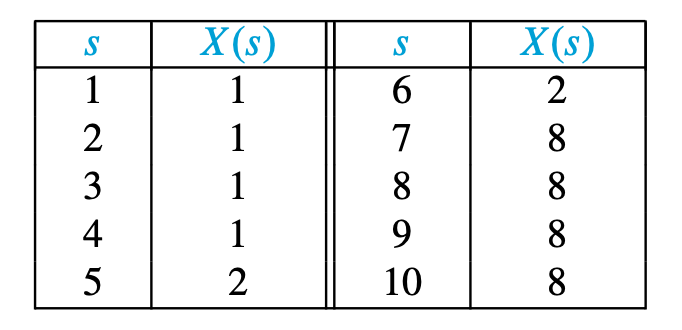
\includegraphics[width=.5\textwidth]{images/center_of_mass__table}
\end{figure}
\vfill 
Now we make a seesaw, placing a weight $P(X=a)$ for each outcome $a$ that the random variable can take on:
\begin{figure}
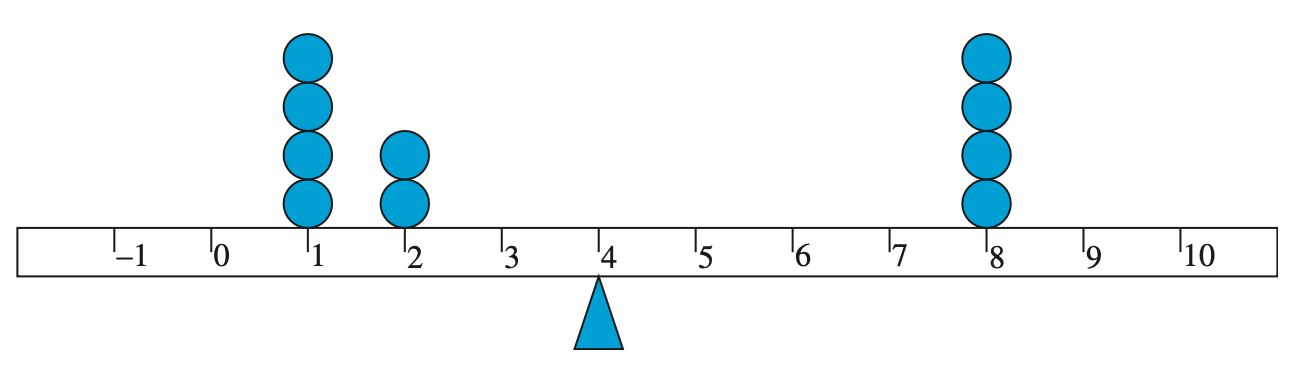
\includegraphics[width=.7\textwidth]{images/center_of_mass}
\end{figure}
%
What is the expected value? \pause The \textbf{balancing point} (\tikz[baseline=-0.5ex]{
    \fill[blue!80] (0,-0.2) -- (0.4,-0.2) -- (0.2,0.35) -- cycle;
}) of the seesaw!

\end{frame}

\begin{frame}{Expectation as center of probability mass}

\begin{figure}
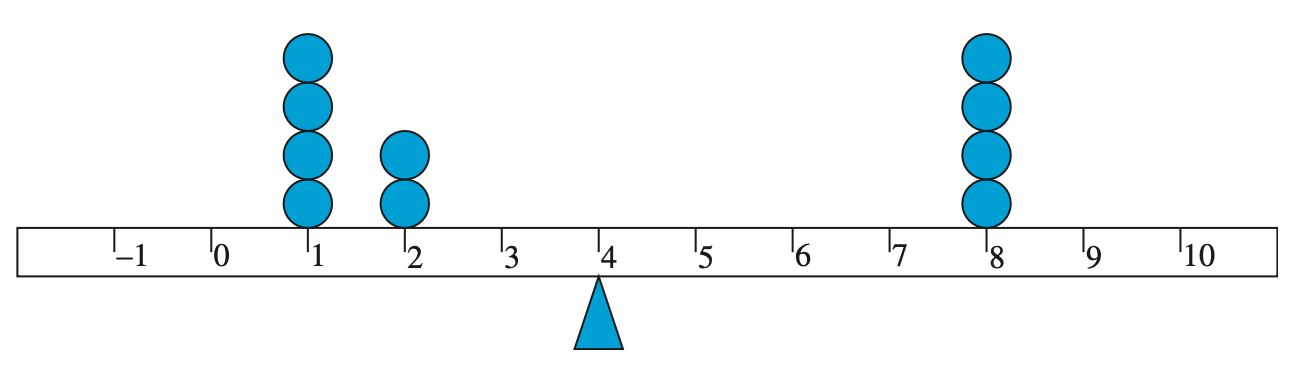
\includegraphics[width=.7\textwidth]{images/center_of_mass}
\end{figure}
\vfill 

To be concrete, the expected value for this problem is given by 
%
\begin{align*}
E[X] &= \sum_{a \in \R} a \, P(X=a) \\
&= 1 \times 0.4 + 2 \times 0.2 + 8 \times 0.4 \\
&= 4 
\end{align*}


\end{frame}


\begin{frame}{Variance as measure of spread}
\footnotesize 
\begin{mygreenbox}[title=Definition]
Let $X$ be a real-valued random variable on a probability space $(S,P)$. Let $\mu \defeq E[X]$.  Then the \textbf{variance} of $X$ is
\[ \Var(X) = \E \big[ (X - \mu)^2 \big] \]
\end{mygreenbox}

\vfill 

\begin{myredbox}[title=Remark]
The variance is the \textbf{expected squared deviation} from the mean. 
\end{myredbox}
\vfill 
\begin{figure}
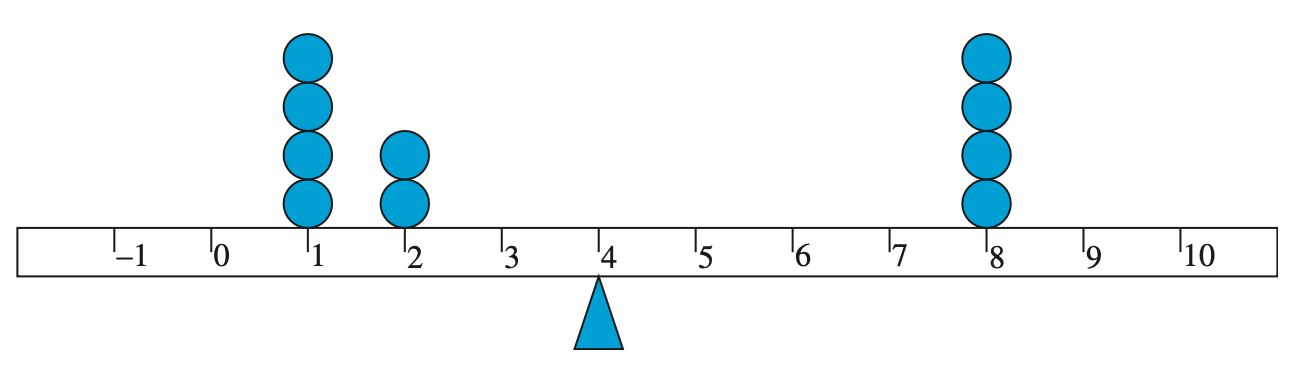
\includegraphics[width=.7\textwidth]{images/center_of_mass}
\end{figure}

\pause 
\vfill 
\colorbox{yellow!30}{\textbf{Poll.}} Can anybody here explain how to compute the variance for this problem? 
\end{frame}


\begin{frame}{Expectation vs. variance}
\footnotesize 
\begin{figure}
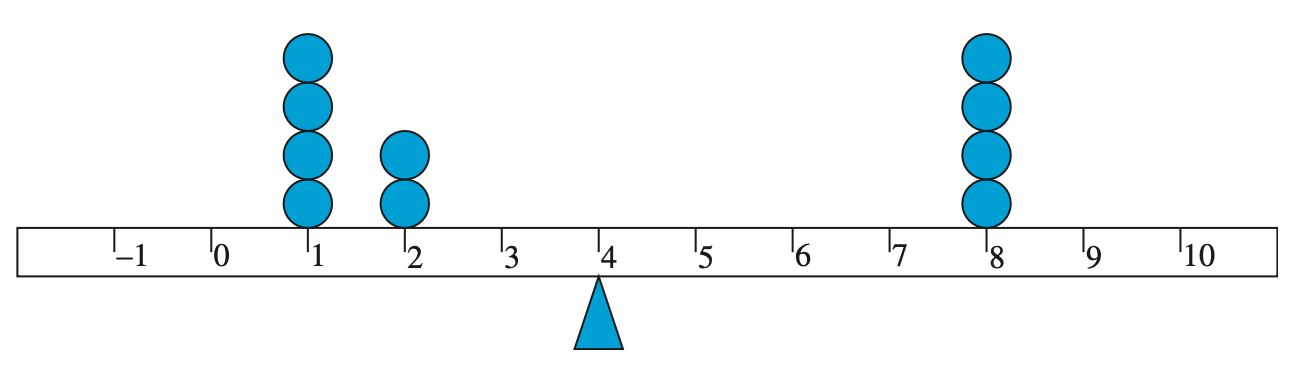
\includegraphics[width=.7\textwidth]{images/center_of_mass}
\end{figure}
\vfill 

Here, the \textbf{expected value} $E[X]$ (a.k.a. the mean $\mu$) is given by 
%
\begin{align*}
E[X] &= \sum_{a \in \R} \colorbox{yellow!30}{$a$} \, P(X=a) \\
&= \colorbox{yellow!30}{1} \times 0.4 + \colorbox{yellow!30}{2} \times 0.2 + \colorbox{yellow!30}{8} \times 0.4 \\
&= 4 
\end{align*}
%
The \textbf{variance} $Var(X)$ (i.e. the expected squared deviation) is given by 
%
\begin{align*}
Var(X) &= \sum_{a \in \R} \colorbox{red!30}{$(a - \mu)^2$} \; P(X=a) \\
 &=\colorbox{red!30}{(1-4)^2} \times 0.4 + \colorbox{red!30}{(2-4)^2} \times 0.2 + \colorbox{red!30}{(8-4)^2} \times 0.4 \\
&= 9 \times 0.4 + 4 \times 0.2 + 16 \times 0.4 \\
&= 10.8
\end{align*}
%

\end{frame}

\begin{frame}
\footnotesize 

\begin{myredbox}[title=Remark]
When computing the variance, we can use
%
\begin{align*}
\Var(X) &= \sum_{s \in S} [X(s) - \mu]^2 \; P(s)  \\
\intertext{or}
&= \sum_{a \in \R} (a - \mu)^2 \; P(X=a)
\end{align*}
\end{myredbox}

\vfill 
\begin{figure}
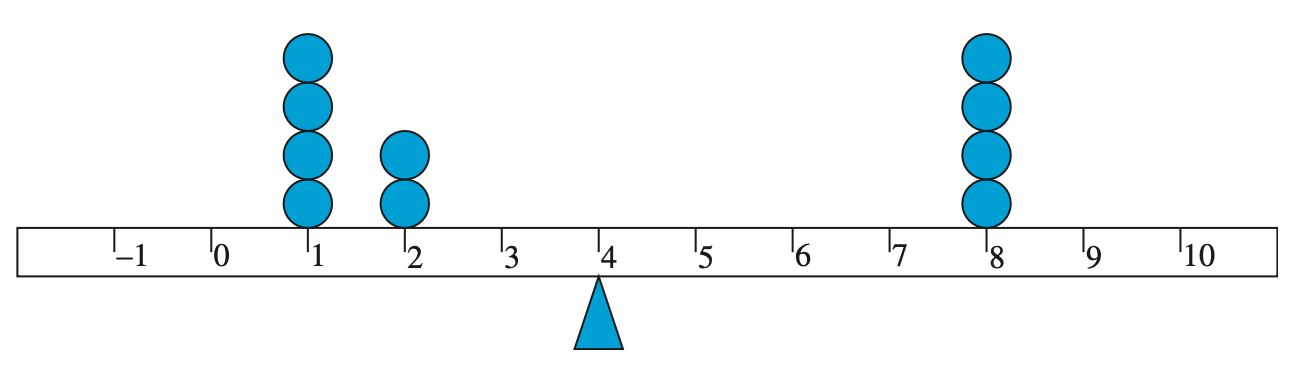
\includegraphics[width=.7\textwidth]{images/center_of_mass}
\end{figure}

\pause 
\vfill 
\colorbox{yellow!30}{\textbf{Poll.}} Can anybody explain how two apply these different methods to this problem?
\end{frame}



\begin{frame}{Three Random Variables}

\colorbox{yellow!30}{\textbf{Poll.}} These three random variables all have the same mean.  Which has the largest variance?
\vfill 
\centering
% Automatically scale to fit the width
\resizebox{\textwidth}{!}{
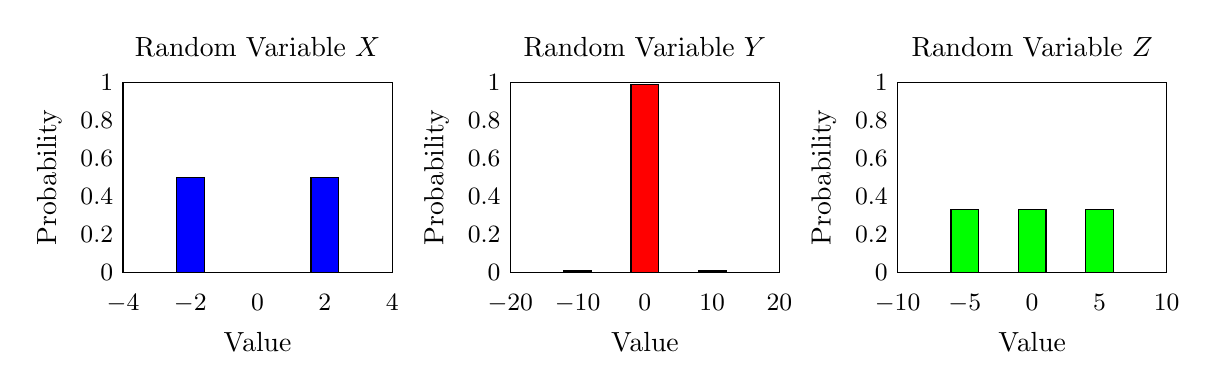
\begin{tikzpicture}
    % Group plots side by side
    \begin{groupplot}[
        group style={group size=3 by 1, horizontal sep=1.5cm},
        width=5cm, height=4cm,
        ybar,
        ymin=0, ymax=1,
        enlarge x limits=0.5,
        ylabel={Probability},
        xlabel={Value},
        xtick style={draw=none},
        ytick style={draw=none},
        xticklabel style={font=\small},
        yticklabel style={font=\small},
    ]

    % Histogram for X
    \nextgroupplot[title={Random Variable \(X\)}]
    \addplot[fill=blue] coordinates {(-2, 0.5) (2, 0.5)};

    % Histogram for Y
    \nextgroupplot[title={Random Variable \(Y\)}]
    \addplot[fill=red] coordinates {(-10, 0.01) (0, 0.99) (10, 0.01)}; 


    % Histogram for Z
    \nextgroupplot[title={Random Variable \(Z\)}]
    \addplot[fill=green] coordinates {(-5, 0.333) (0, 0.333) (5, 0.333)};

    \end{groupplot}
\end{tikzpicture}
}
\vfill
\pause 
\colorbox{blue!30}{\textbf{Solution.}} $Z$ has the largest variance. (See textbook for more info.)
 


\end{frame}

\begin{frame}[standout]
Group exercises
\end{frame}

\begin{frame}
\footnotesize 
\vfill 
\begin{columns}
\begin{column}{0.33\textwidth}
aaron.loomis: 16 \\ 
adam.wyszynski: 9 \\ 
alexander.goetz: 8 \\ 
alexander.knutson: 14 \\ 
anthony.mann: 4 \\ 
blake.leone: 10 \\ 
bridger.voss: 12 \\ 
caitlin.hermanson: 19 \\ 
cameron.wittrock: 5 \\ 
carsten.brooks: 18 \\ 
carver.wambold: 20 \\ 
colter.huber: 8 \\ 
conner.reed1: 7 \\ 
connor.mizner: 17 \\ 
connor.yetter: 5 \\ 
derek.price4: 19 \\ 
devon.maurer: 1 \\ 
emmeri.grooms: 7 \\ 
erik.moore3: 15 \\ 
ethan.johnson18: 20 \\ 
evan.barth: 15 \\\end{column}
\begin{column}{0.33\textwidth}
evan.schoening: 1 \\ 
griffin.short: 8 \\ 
jack.fry: 17 \\ 
jacob.ketola: 21 \\ 
jacob.ruiz1: 9 \\ 
jacob.shepherd1: 14 \\ 
jada.zorn: 12 \\ 
jakob.kominsky: 10 \\ 
james.brubaker: 21 \\ 
jeremiah.mackey: 17 \\ 
jett.girard: 11 \\ 
john.fotheringham: 12 \\ 
jonas.zeiler: 6 \\ 
joseph.mergenthaler: 16 \\ 
joseph.triem: 16 \\ 
julia.larsen: 3 \\ 
justice.mosso: 15 \\ 
kaden.price: 5 \\ 
lucas.jones6: 3 \\ 
luka.derry: 11 \\ 
luke.donaldson1: 11 \\\end{column}
\begin{column}{0.33\textwidth}
lynsey.read: 7 \\ 
mason.barnocky: 4 \\ 
matthew.nagel: 21 \\ 
micaylyn.parker: 13 \\ 
michael.oswald: 14 \\ 
nolan.scott1: 2 \\ 
owen.obrien: 3 \\ 
pendleton.johnston: 20 \\ 
peter.buckley1: 18 \\ 
reid.pickert: 2 \\ 
ryan.barrett2: 19 \\ 
samuel.hemmen: 13 \\ 
samuel.mosier: 6 \\ 
samuel.rollins: 9 \\ 
sarah.periolat: 2 \\ 
timothy.true: 4 \\ 
tristan.nogacki: 13 \\ 
tyler.broesel: 10 \\ 
william.elder1: 1 \\ 
yebin.wallace: 18 \\ 
zeke.baumann: 6 \\\end{column}
\end{columns}
\vfill
\end{frame}

\begin{frame}{Group exercises}
\footnotesize 
\begin{enumerate}
	\item \textit{Simplified stock market.} Suppose there are three kinds of days: \texttt{GOOD}, \texttt{GREAT}, and \texttt{ROTTEN}. The following chart gives the frequency of each of these types of days and the effect on the price (in dollars) of a certain stock that day.
	
	\begin{table}[H]
	\begin{tabular}{|c|c|c|}
	\toprule 
	\colorbox{blue!30}{Type of day} & 	\colorbox{blue!30}{Frequency} & \colorbox{blue!30}{Change in stock value} \\
	\midrule 
	\texttt{GOOD} & 60\% & +2 \\
	\texttt{GREAT} & 10\% & +5 \\
	\texttt{ROTTEN} & 30\% & -4 \\
	\bottomrule 
	\end{tabular}
	\end{table}
	
	Let $X_n$ be the change in the value of the stock after $n$ consecutive days.
	 \begin{itemize} \footnotesize 
	\item[a.] Find $E[X_1]$, the expected change in stock price after one day. 
	\item[b.] Find  $Var[X_1]$, the variance in the change in stock price after one day. 
	\item[c.] Find $E[X_5]$.
	\item[d.] Find $Var[X_5]$.
	\end{itemize}
	\vspace{-.2cm}
	\item  \leavevmode
	\begin{minipage}{.70\textwidth}
	\footnotesize  A pair of 25-sided dice is rolled. Let $X$ be the sum of the two numbers and $Y$ be the product. Find $E[X]$ and $E[Y]$.
	\end{minipage} %
	\hfill 
	\begin{minipage}{.15\textwidth}
	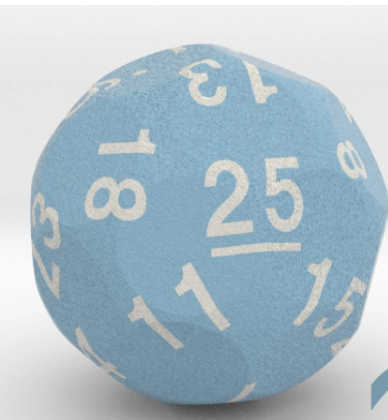
\includegraphics[width=.7\linewidth]{images/25_sided_die}
	\end{minipage}
	\vspace{-.1cm}
	\item  The term \textit{expected value} can be a bit deceiving. Sometimes it is not what someone might expect! (a) Give an example of a random variable $X$ where $E[X]=1$ but $P(X=1)=0$.  (b) Give an example of a random variable $X$ where $E[X]<0$ but the probability that $X$ is positive is nearly 100\%.
\end{enumerate}

\end{frame}


\begin{frame}{Solution to group exercise \#1a}
\footnotesize 

\textbf{Problem \& Solution.} \textit{Simplified stock market.} Suppose there are three kinds of days: \texttt{GOOD}, \texttt{GREAT}, and \texttt{ROTTEN}. The following chart gives the frequency of each of these types of days and the effect on the price (in dollars) of a certain stock that day.
	\vspace{-.2cm}
	\begin{table}[H]
	\begin{tabular}{|c|c|c|}
	\toprule 
	\colorbox{blue!30}{Type of day} & 	\colorbox{blue!30}{Frequency} & \colorbox{blue!30}{Change in stock value} \\
	\midrule 
	\texttt{GOOD} & 60\% & +2 \\
	\texttt{GREAT} & 10\% & +5 \\
	\texttt{ROTTEN} & 30\% & -4 \\
	\bottomrule 
	\end{tabular}
	\end{table}
	\vspace{-.2cm}
	Let $X_n$ be the change in the value of the stock after $n$ consecutive days.
		%
		\vspace{-.2cm}
		%
	 \begin{itemize} \footnotesize 
	\item[a.] Find $E[X_1]$, the expected change in stock price after one day. 
	%
	\begin{align*}
	 E[X_1] &= \sum_{s \in S} X_1(s) P(s)  \\
	 &= (+2)(0.6) + 	(+5)(0.1) + (-4)(.30) = 0.5
	\end{align*}
	%
	We expect the stock value to rise \$0.50 after one day.
	\end{itemize}
\end{frame}


\begin{frame}{Solution to group exercise \#1b}
\footnotesize 

\textbf{Problem \& Solution.} \textit{Simplified stock market.} Suppose there are three kinds of days: \texttt{GOOD}, \texttt{GREAT}, and \texttt{ROTTEN}. The following chart gives the frequency of each of these types of days and the effect on the price (in dollars) of a certain stock that day.
	\vspace{-.2cm}
	\begin{table}[H]
	\begin{tabular}{|c|c|c|}
	\toprule 
	\colorbox{blue!30}{Type of day} & 	\colorbox{blue!30}{Frequency} & \colorbox{blue!30}{Change in stock value} \\
	\midrule 
	\texttt{GOOD} & 60\% & +2 \\
	\texttt{GREAT} & 10\% & +5 \\
	\texttt{ROTTEN} & 30\% & -4 \\
	\bottomrule 
	\end{tabular}
	\end{table}
	\vspace{-.2cm}
	Let $X_n$ be the change in the value of the stock after $n$ consecutive days.
		%
		\vspace{-.2cm}
		%
	 \begin{itemize} \footnotesize 
	\item[b.] Find  $Var[X_1]$, the variance in the change in stock price after one day.
	%
	\begin{align*}
	 Var[X_1] &= \sum_{s \in S} (X_1(s)-\mu)^2 P(s)  && \text{(where $\mu \defeq \E[X_1]$)} \\
	 \intertext{Since we know from part (a) that $\mu=0.5$,}
	 &= \sum_{s \in S} (X_1(s)-0.5)^2 P(s) \\
	 &= (2 - 0.5)^2 \times .6 + 	(5-0.5)^2 \times .3 + (-4-0.5)^2 \times .10 \\
	 &= 9.45
	\end{align*}
	\end{itemize}
\end{frame}


\begin{frame}{Solution to group exercise \#1b -- Alternate solution.}
\footnotesize 

\textbf{Problem \& Solution.} \textit{Simplified stock market.} Suppose there are three kinds of days: \texttt{GOOD}, \texttt{GREAT}, and \texttt{ROTTEN}. The following chart gives the frequency of each of these types of days and the effect on the price (in dollars) of a certain stock that day.
	\vspace{-.2cm}
	\begin{table}[H]
	\begin{tabular}{|c|c|c|}
	\toprule 
	\colorbox{blue!30}{Type of day} & 	\colorbox{blue!30}{Frequency} & \colorbox{blue!30}{Change in stock value} \\
	\midrule 
	\texttt{GOOD} & 60\% & +2 \\
	\texttt{GREAT} & 10\% & +5 \\
	\texttt{ROTTEN} & 30\% & -4 \\
	\bottomrule 
	\end{tabular}
	\end{table}
	\vspace{-.2cm}
	Let $X_n$ be the change in the value of the stock after $n$ consecutive days.
		%
		\vspace{-.2cm}
		%
	 \begin{itemize} \footnotesize 
	\item[b.] Find  $Var[X_1]$, the variance in the change in stock price after one day.
	%
	\begin{align*}
	 Var[X_1] &= E[X_1^2] - E[X_1]^2
	 \end{align*}
	 %
	For the first summand,  
	%
	\begin{align*}
	E[X_1^2] &= \sum_{s \in S} X_1(s) P(s)  \\
	 &= (+2)^2 \times .6 + 	(+5)^2 \times .3 + (-4)^2 \times .10 = 0.5 \\
	 &= 4 \times .6 + 	25 \times .3 + 16 \times .10 = 9.7 
	 \end{align*}
	 %
	 For the second summand, we know  from part (a) that $\E[X_1]=0.5$. Hence $\E[X_1]^2=0.25$.  Putting this together, we have
	 \[  Var[X_1] = E[X_1^2] - E[X_1]^2 = 9.7-0.25 = 9.45.\]
	\end{itemize}
\end{frame}


\begin{frame}{Solution to group exercise \#1c}
\footnotesize 

\textbf{Problem \& Solution.} \textit{Simplified stock market.} Suppose there are three kinds of days: \texttt{GOOD}, \texttt{GREAT}, and \texttt{ROTTEN}. The following chart gives the frequency of each of these types of days and the effect on the price (in dollars) of a certain stock that day.
	\vspace{-.2cm}
	\begin{table}[H]
	\begin{tabular}{|c|c|c|}
	\toprule 
	\colorbox{blue!30}{Type of day} & 	\colorbox{blue!30}{Frequency} & \colorbox{blue!30}{Change in stock value} \\
	\midrule 
	\texttt{GOOD} & 60\% & +2 \\
	\texttt{GREAT} & 10\% & +5 \\
	\texttt{ROTTEN} & 30\% & -4 \\
	\bottomrule 
	\end{tabular}
	\end{table}
	\vspace{-.2cm}
	Let $X_n$ be the change in the value of the stock after $n$ consecutive days.
		%
		\vspace{-.2cm}
		%
	 \begin{itemize} \footnotesize 
	\item[c.] Find $E[X_5]$, the expected change in stock price after five days. 
	%
	The analysis is simplest if we write $X_5 = Y_1 + Y_2 + \hdots + Y_5$, where $Y_j$ is the change in stock price on the $j$-th day. \\
	
	Now, by linearity of expectation
	\[E[X_5] = E[Y_1] + E[Y_2] + \hdots + E[Y_5].\] 
	 %
	 Each summand is given by
	 \[E[Y_j] = (+2)(0.6) + 	(+5)(0.1) + (-4)(.30) = 0.5, \]
	 as was solved in part (a).
	 
	 Hence, 
	 \[E[X_5] = 5(0.5) = 2.5 \]
	  %
	  We expect the stock value to rise \$2.50 after 5 days.
	\end{itemize}
\end{frame}

\begin{frame}{Solution to group exercise \#1d.}
\footnotesize
\textbf{Problem.}  Find $Var[X_5]$, the variance of the change in stock price after five days. 
\vfill \vfill 
\textbf{Solution.}   We write
  \[ Var[X_5] = E[X_5^2] - E[X_5]^2 \]
  For the second summand, we know from part (c) that $E[X_5] = 2.5$, so $ E[X_5]^2 = 2.5^2 = 6.25$. \\
   \vfill 
   For the first summand, we again write $X_5 = Y_1 + Y_2 + \hdots + Y_5$, where $Y_j$ is the change in stock price on the $j$-th day.  We use the fact that the $Y_j$'s are independent.
   %
   \begin{align*}
   E[X_5^2] &= E[(Y_1 + Y_2 + \hdots + Y_5)^2] \\
   &=E[Y_1^2 + \hdots + Y_5^2 + 2Y_1Y_2 + \hdots +2Y_4Y_5] && \scripttext{(expanding the sum of squares)}\\
   &= 5E[Y_1^2] + 20E[Y_1Y_2] && \scripttext{(since $Y_j$'s are identical)}\\
   &= 5E[Y_1^2] + 20E[Y_1]E[Y_2]  && \scripttext{(by independence)}\\
   &= (5)(9.7)  + 20(0.5)^2 && \scripttext{(using previous parts)}\\
   &= 53.5
   \end{align*}

Hence,
  \[ Var[X_5] = E[X_5^2] - E[X_5]^2 = 53.5 - 6.25 = 47.25 \]
\vfill \vfill 
\textbf{Remark.} This problem is much simpler if we use a fact (not presented in the text) that 
\[ Var(X_5) = Var(Y_1) + \hdots Var(Y_5)\]
because the $Y_j$'s are independent.
\end{frame}



\end{document}
